\documentclass[14pt, a4paper]{article}
\usepackage[utf8]{inputenc}
\usepackage[russian]{babel}
\usepackage{graphicx}

\title{\textbf{Отчет о выполнении лабораторной работы 1.1.3}}
\author{Калашников Михаил, Б03-205}
\date{}

\begin{document}

\maketitle

При выполнении лабораторной работы использовался набор из 270 резисторов, имеющих номинальное сопротивление $500\ \Omega$ и цифровой мультиметр.
\par
Результаты измерений сопротивлений всех 270 резисторов (в $\Omega$) приводятся в таблице \ref{table1}. Значения отсортированы в порядке неубывания.
\par
По значениям из таблицы \ref{table1} строим гистограммы для $m=20$ и $m=10$. Для удобства сравнения полученного распределения с нормальным, по оси ординат откладывается число измерений $\Delta n$, попавших в данный интервал отнесенное к общему количеству измерений $N$ и к величине интервала $\Delta R=\frac{R_{max}-R_{min}}{m}$. В таблицах \ref{table2} и \ref{table3} в зависимости от номера группы $k$ приведены значения $\Delta n$ и $\omega=\frac{\Delta n}{N\Delta R}$. На рисунках \ref{image1} и \ref{image2} представлены гистограммы. Среднее значение $R_{av}$ найдено по формуле:
\[R_{av}=\frac{1}{N}\sum_{i=1}^{N}R_i=499.4\ \Omega.\]
\par
Среднеквадратичное отклонение найдено по формуле:
\[\sigma=\sqrt{\frac{1}{N}\sum_{i=1}^{N}\left(R_i-R_{av}\right)^2}\approx1.3\ \Omega.\]
\par
Эта функция также изображена на рисунках \ref{image1} и \ref{image2}. Видно, что гистограмма соответствует данной зависимости. Теоретическая вероятность попадания измерений в интервал от $R_{av}-\sigma$ до $R_{av}+\sigma$ равна 68\%, а в интервал от $R_{av}-2\sigma$ до $R_{av}+2\sigma$ -- 95\%.
\par
Из проведенной работы мы получаем, что сопротивление наугад выбранного сопротивления попадет в интервал $500\pm1.3\ \Omega$ с вероятностью в 71\%, в интервал $500\pm2.6\ \Omega$ – с вероятностью 95\%, а в интервал $500\pm3.9\ \Omega$ – с вероятностью 99\%.

\begin{table}
\centering
\begin{tabular}{c c c c c c c c c}

496.3 & 496.6 & 496.8 & 496.9 & 496.9 & 496.9 & 497.3 & 497.4 & 497.5 \\
497.5 & 497.5 & 497.5 & 497.6 & 497.6 & 497.7 & 497.7 & 497.7 & 497.7 \\
497.7 & 497.7 & 497.7 & 497.7 & 497.7 & 497.8 & 497.8 & 497.8 & 497.8 \\
497.8 & 497.9 & 497.9 & 497.9 & 497.9 & 498.0 & 498.0 & 498.0 & 498.0 \\
498.0 & 498.0 & 498.1 & 498.1 & 498.1 & 498.1 & 498.1 & 498.1 & 498.1 \\
498.2 & 498.2 & 498.2 & 498.2 & 498.3 & 498.3 & 498.3 & 498.3 & 498.4 \\
498.4 & 498.4 & 498.4 & 498.4 & 498.4 & 498.4 & 498.5 & 498.5 & 498.5 \\
498.5 & 498.5 & 498.5 & 498.5 & 498.5 & 498.5 & 498.5 & 498.5 & 498.6 \\
498.6 & 498.6 & 498.6 & 498.6 & 498.7 & 498.7 & 498.7 & 498.7 & 498.7 \\
498.8 & 498.8 & 498.8 & 498.8 & 498.8 & 498.8 & 498.8 & 498.8 & 498.8 \\
498.8 & 498.8 & 498.8 & 498.8 & 498.8 & 498.9 & 498.9 & 498.9 & 498.9 \\
498.9 & 498.9 & 498.9 & 498.9 & 498.9 & 498.9 & 498.9 & 498.9 & 499.0 \\
499.0 & 499.0 & 499.0 & 499.0 & 499.0 & 499.0 & 499.0 & 499.0 & 499.0 \\
499.0 & 499.0 & 499.1 & 499.1 & 499.1 & 499.1 & 499.1 & 499.1 & 499.1 \\
499.1 & 499.1 & 499.1 & 499.2 & 499.2 & 499.2 & 499.2 & 499.2 & 499.2 \\
499.2 & 499.2 & 499.2 & 499.3 & 499.3 & 499.3 & 499.3 & 499.3 & 499.3 \\
499.3 & 499.3 & 499.3 & 499.3 & 499.3 & 499.3 & 499.3 & 499.4 & 499.4 \\
499.4 & 499.4 & 499.4 & 499.4 & 499.4 & 499.4 & 499.4 & 499.5 & 499.5 \\
499.5 & 499.5 & 499.5 & 499.5 & 499.5 & 499.5 & 499.6 & 499.6 & 499.6 \\
499.6 & 499.6 & 499.7 & 499.7 & 499.7 & 499.7 & 499.7 & 499.7 & 499.7 \\
499.7 & 499.7 & 499.8 & 499.8 & 499.8 & 499.8 & 499.8 & 499.8 & 499.8 \\
499.8 & 499.8 & 499.9 & 499.9 & 500.0 & 500.0 & 500.0 & 500.0 & 500.0 \\
500.0 & 500.0 & 500.0 & 500.0 & 500.1 & 500.1 & 500.1 & 500.1 & 500.1 \\
500.1 & 500.2 & 500.3 & 500.3 & 500.3 & 500.3 & 500.3 & 500.3 & 500.3 \\
500.4 & 500.4 & 500.4 & 500.4 & 500.4 & 500.4 & 500.4 & 500.4 & 500.4 \\
500.4 & 500.5 & 500.6 & 500.6 & 500.6 & 500.7 & 500.7 & 500.7 & 500.8 \\
500.8 & 500.8 & 500.8 & 500.9 & 500.9 & 500.9 & 500.9 & 500.9 & 500.9 \\
501.0 & 501.0 & 501.0 & 501.1 & 501.2 & 501.2 & 501.2 & 501.3 & 501.3 \\
501.3 & 501.4 & 501.6 & 501.7 & 501.7 & 501.7 & 501.8 & 501.9 & 502.1 \\
502.1 & 502.4 & 502.4 & 502.5 & 502.5 & 502.6 & 502.8 & 503.7 & 505.1 \\

\end{tabular}
\caption{Результаты измерения сопротивления 270 резисторов}
\label{table1}
\end{table}

\begin{table}
\centering
\begin{tabular}{| c | c | c | c | c | c | c | c | c | c | c |}
\hline
$k$ & 1 & 2 & 3 & 4 & 5 & 6 & 7 & 8 & 9 & 10 \\
\hline
$\Delta n$ & 2 & 4 & 8 & 24 & 33 & 36 & 44 & 40 & 18 & 24 \\
\hline
$\omega\cdot1000, \Omega^{-1}$ & 17 & 34 & 67 & 202 & 278 & 303 & 370 & 337 & 152 & 202 \\
\hline
\hline
$k$ & 11 & 12 & 13 & 14 & 15 & 16 & 17 & 18 & 19 & 20 \\
\hline
$\Delta n$ & 14 & 7 & 6 & 4 & 4 & 0 & 1 & 0 & 0 & 1 \\
\hline
$\omega\cdot1000, \Omega^{-1}$ & 118 & 59 & 51 & 34 & 34 & 0 & 8 & 0 & 0 & 8 \\
\hline
\end{tabular}
\caption{Значения $\Delta n$ и $\omega$ в зависимости от номера группы $k$ для $m=20$}
\label{table2}
\end{table}

\begin{table}
\centering
\begin{tabular}{| c | c | c | c | c | c | c | c | c | c | c |}
\hline
$k$ & 1 & 2 & 3 & 4 & 5 & 6 & 7 & 8 & 9 & 10 \\
\hline
$\Delta n$ & 6 & 32 & 69 & 84 & 42 & 21 & 10 & 4 & 1 & 1 \\
\hline
$\omega\cdot10^3, \Omega^{-1}$ & 25 & 135 & 290 & 354 & 177 & 88 & 42 & 17 & 4 & 4 \\
\hline
\end{tabular}
\caption{Значения $\Delta n$ и $\omega$ в зависимости от номера группы $k$ для $m=10$}
\label{table3}
\end{table}

\begin{figure}
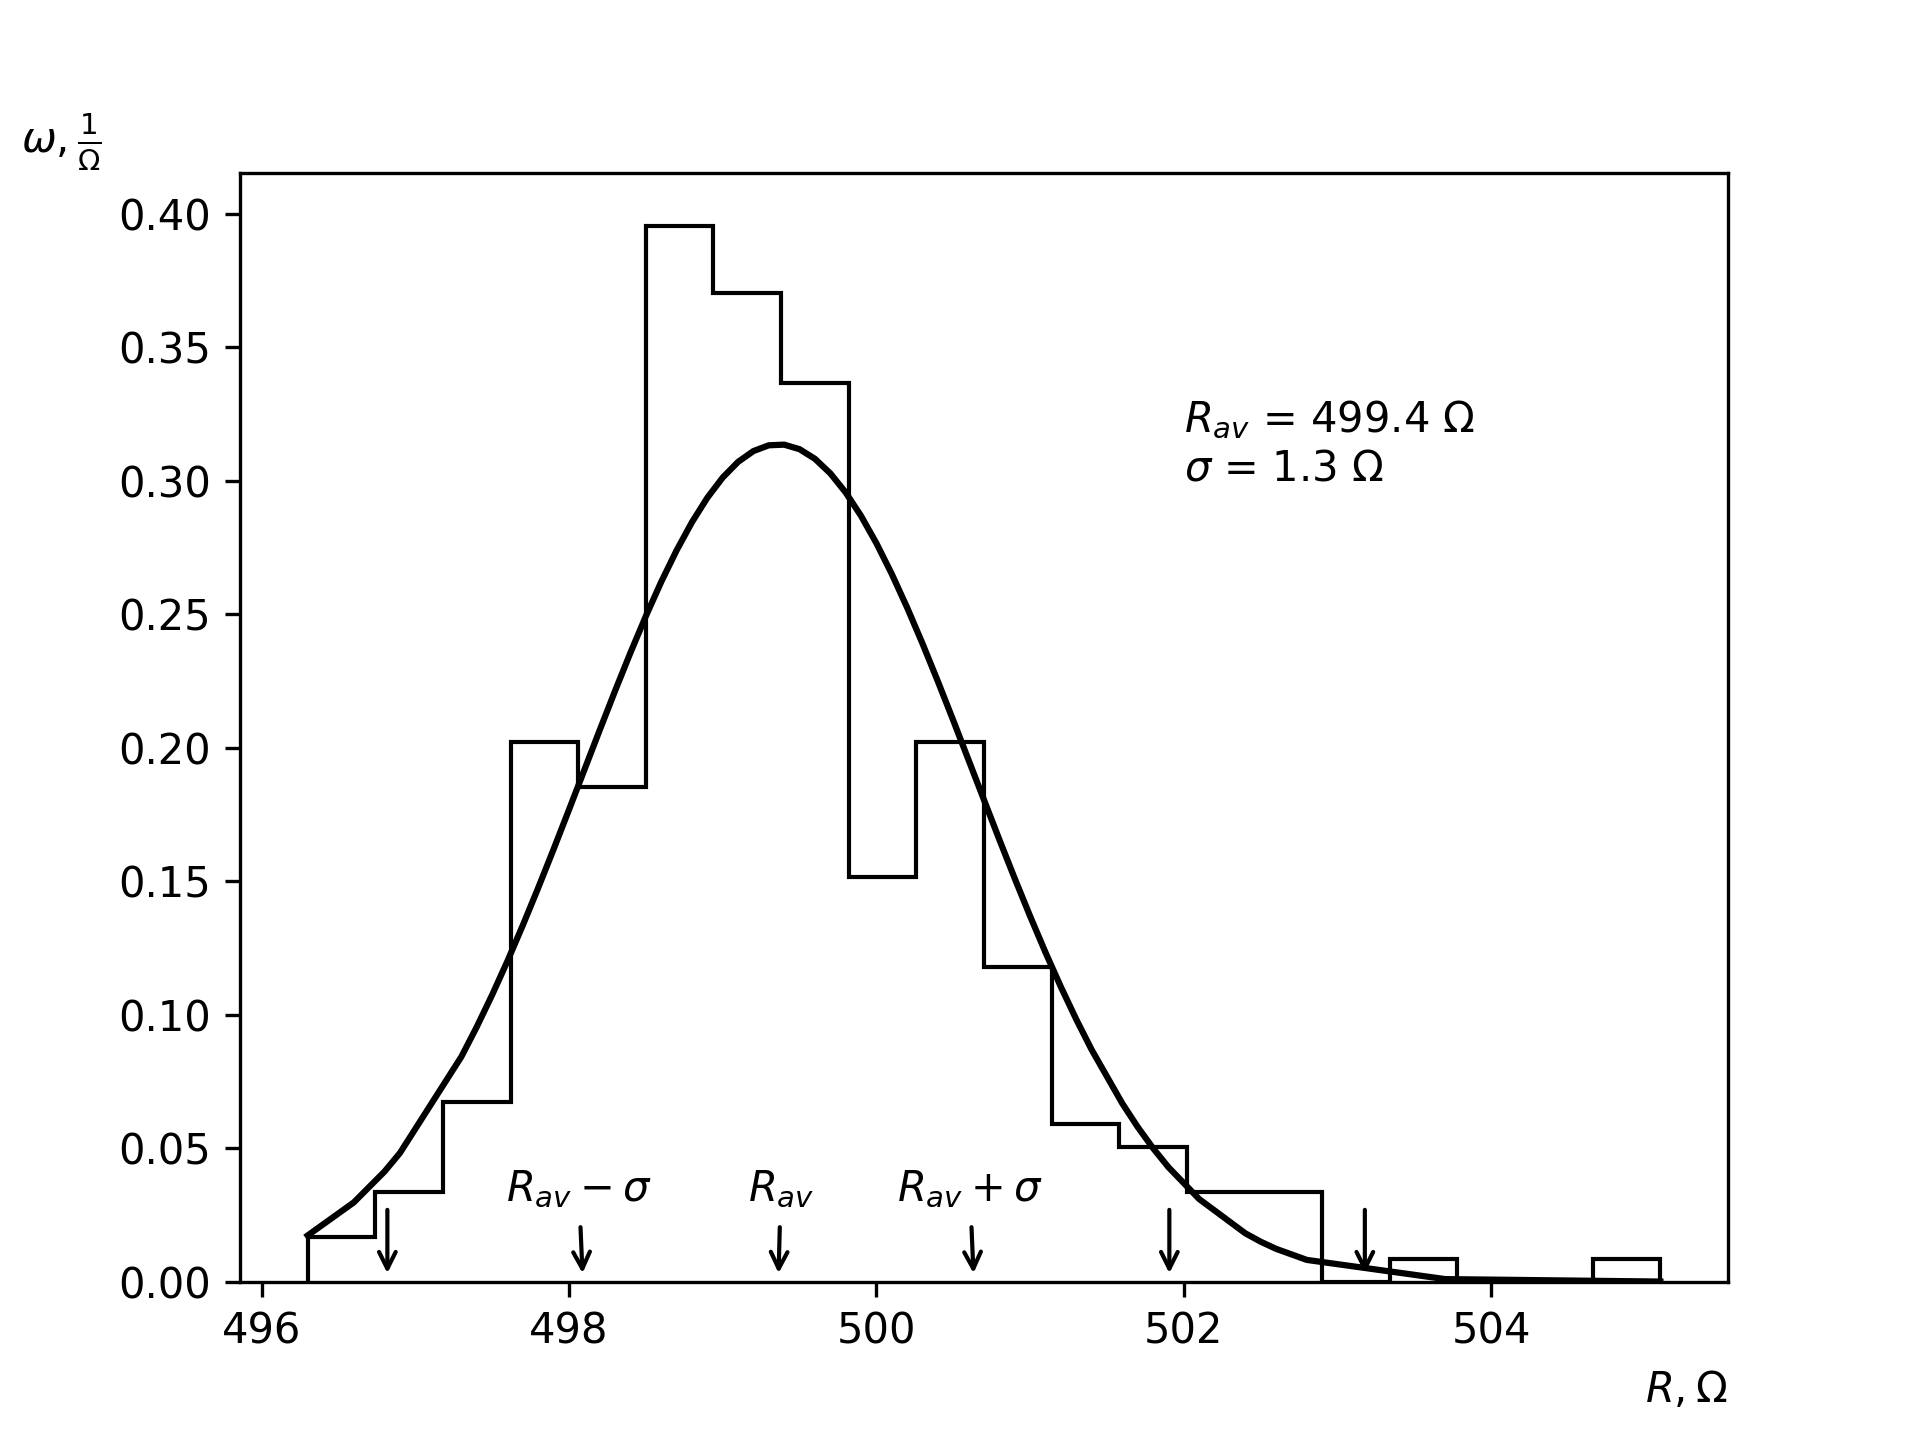
\includegraphics[width=\linewidth]{laba1m20.png}
\caption{Гистограмма для $m=20$}
\label{image1}
\end{figure}

\begin{figure}
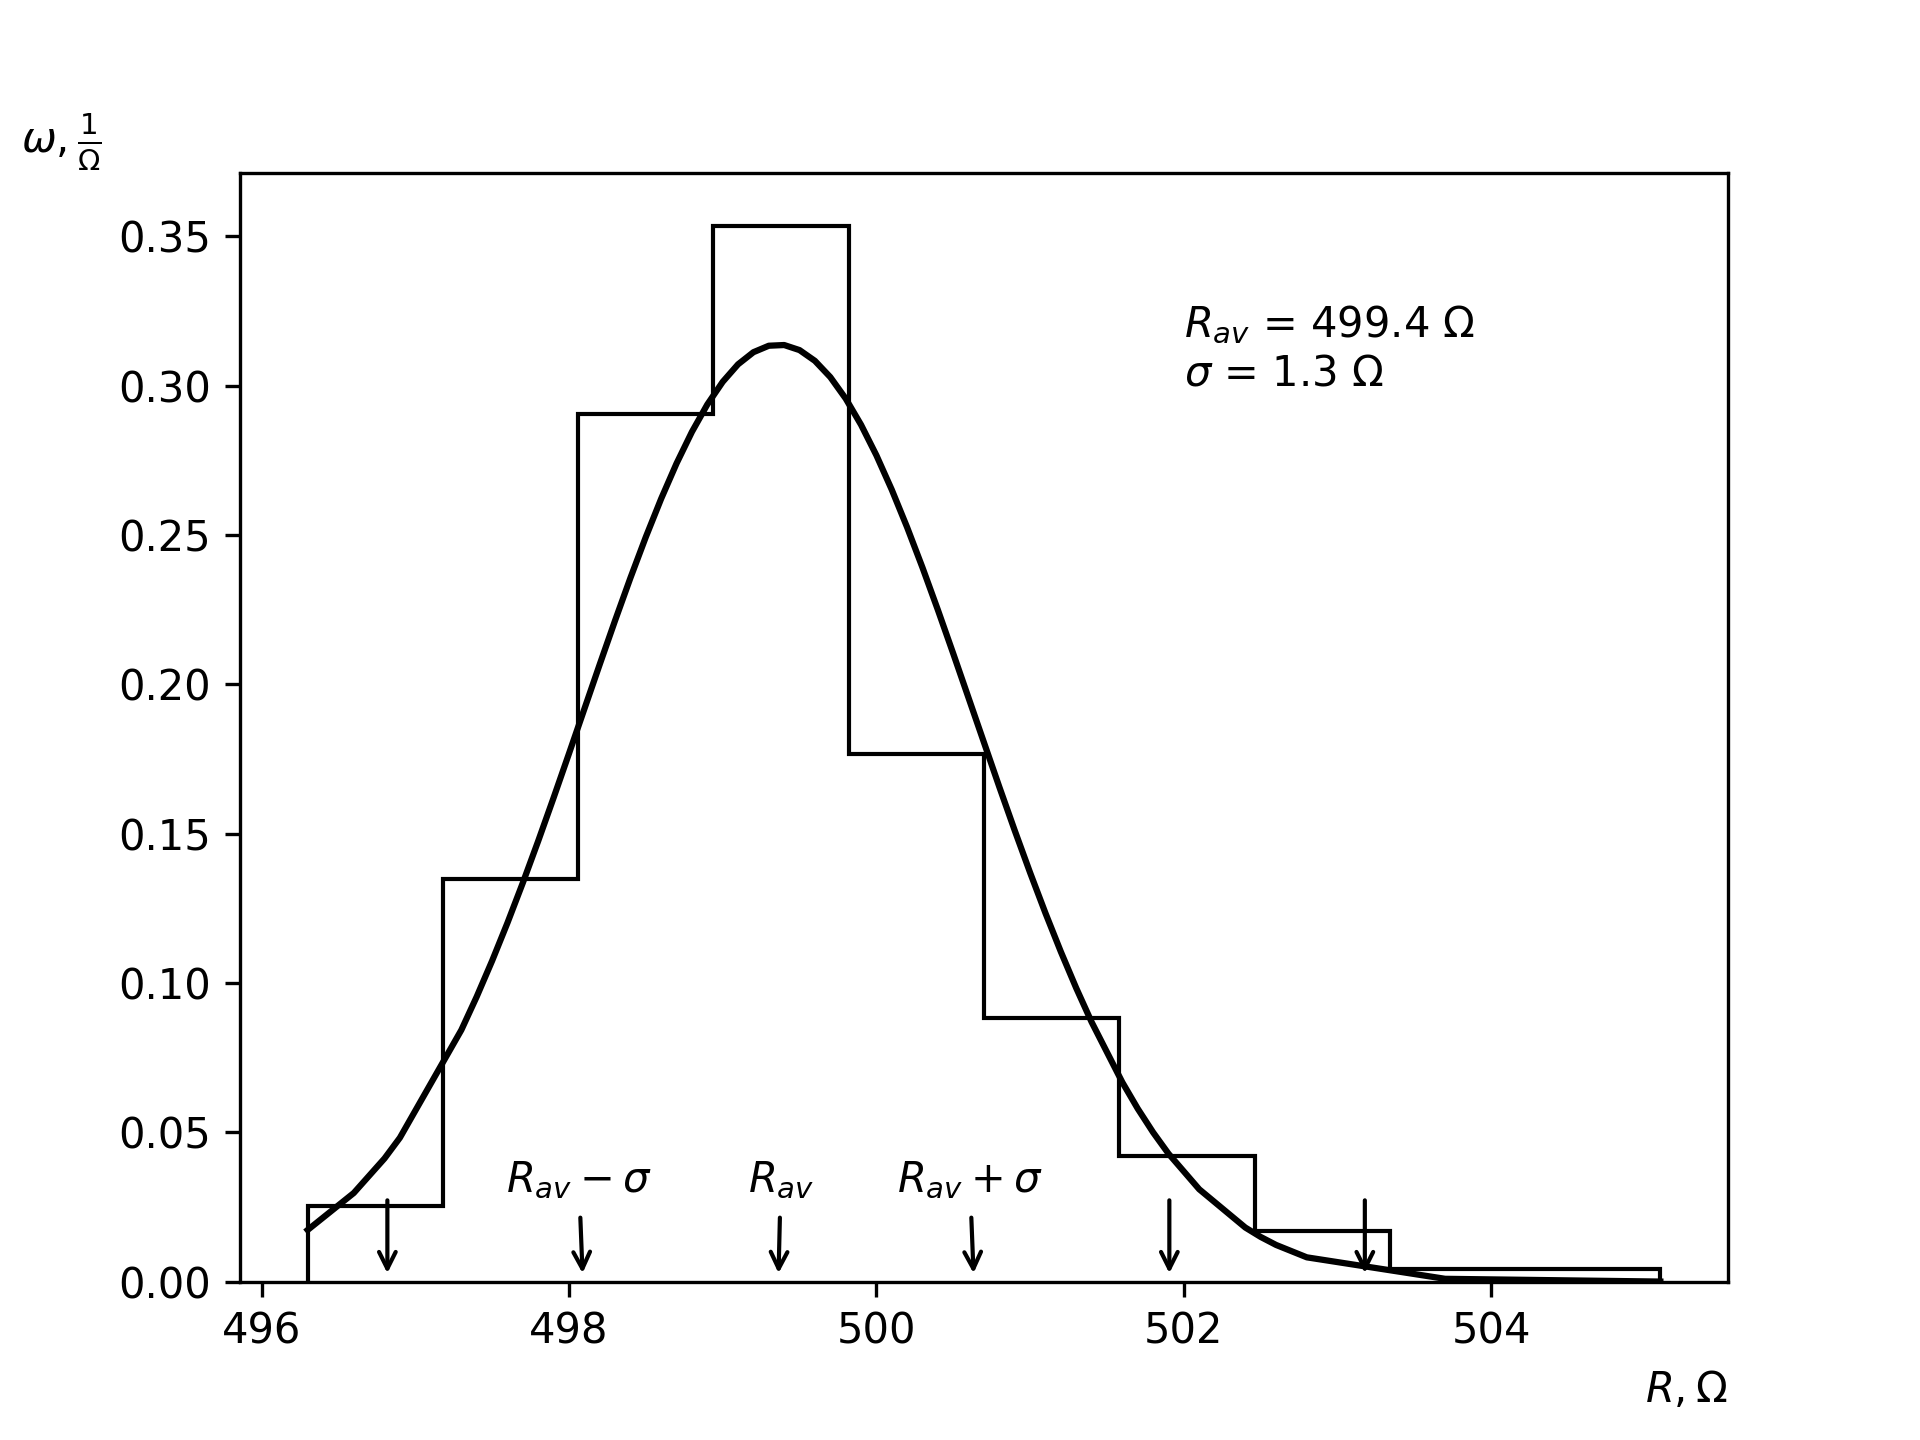
\includegraphics[width=\linewidth]{laba1m10.png}
\caption{Гистограмма для $m=10$}
\label{image2}
\end{figure}

\end{document}